\documentclass[12pt]{article}

\usepackage[a4paper,
mag=1000, includefoot,
left=3cm, right=1.5cm, top=2cm, bottom=2cm, headsep=1cm, footskip=1cm]{geometry}
\usepackage[T2A]{fontenc}
\usepackage[utf8x]{inputenc}
\usepackage[english, main=russian]{babel}
\ifpdf\usepackage{epstopdf}\fi

\usepackage{amsmath,amssymb,amsthm,amscd,amsfonts}
\usepackage{mathdots}
\usepackage{graphicx}
\usepackage{algorithm}
\usepackage{algpseudocode}
\usepackage{algorithmicx}
\usepackage{bbm}
\usepackage{hyperref}
\usepackage{booktabs}
\usepackage{float}

\newcommand\norm[1]{\left\|#1\right\|}
\DeclareMathOperator\R{\mathbb{R}}
\DeclareMathOperator\N{\mathbb{N}}
\DeclareMathOperator\rank{\textrm{rank}\,}


\title{Актуарная математика. Вариант 5\\
	Решение задачи 2 и 4}
\author{\emph{Яковлев Д.М.}\\\textsc{st095998@student.spbu.ru}}
\date{\today}

\begin{document}
	\maketitle
	\section*{Задание 2. Модель Крамера-Лундберга}
	
	\subsection*{Исходные данные}
	По варианту $i = 5$ заданы параметры:
	\begin{itemize}
		\item Интенсивность страховых случаев: $\lambda = 5 + 5 = 10$
		\item Параметры гамма-распределения для исков:
		\begin{itemize}
			\item Форма: $\gamma = 8 + 5 = 13$
			\item Масштаб: $\mu = 4.8$
		\end{itemize}
		\item Нагрузка безопасности: $\delta = 10\% = 0.1$
		\item Целевая вероятность разорения: $\Psi(U) = 0.1$
	\end{itemize}
	
	\subsection*{Пункт 1. Основные расчеты}
	
	\subsubsection*{1. Расчет моментов распределений}
	
	Для отдельного иска $X_i$:
	\begin{align*}
		\mathbb{E}X &= \gamma \mu = 13 \times 4.8 = 62.4 \\
		\mathbb{D}X &= \gamma \mu^2 = 13 \times 23.04 = 299.52
	\end{align*}
	
	Для числа случаев $K$:
	\begin{align*}
		\mathbb{E}K &= \lambda = 10 \\
		\mathbb{D}K &= \lambda = 10
	\end{align*}
	
	Для суммарного иска $Z$:
	\begin{align*}
		\mathbb{E}Z &= \lambda \mathbb{E}X = 10 \times 62.4 = 624 \\
		\mathbb{D}Z &= \lambda((\mathbb{E}X)^2 + \mathbb{D}X) = 10(3893.76 + 299.52) = 41,\!932.8 \\
		\sigma_Z &= \sqrt{\mathbb{D}Z} \approx 204.77
	\end{align*}
	
	\subsubsection*{2. Расчет страховой премии}
	\begin{align*}
		P &= (1+\delta)\mathbb{E}Z = 1.1 \times 624 = 686.4
	\end{align*}
	
	\subsubsection*{3. Оценка параметра $\beta$}
	\begin{align*}
		\beta &\approx \frac{2(P-\mathbb{E}Z)}{\mathbb{D}Z} = \frac{2 \times 62.4}{41,\!932.8} \approx 0.002976
	\end{align*}
	
	\subsubsection*{4. Расчет начального капитала}
	\begin{align*}
		U &= -\frac{\ln \Psi(U)}{\beta} \approx \frac{2.3026}{0.002976} \approx 773.7 \\
		\frac{U}{\mathbb{E}Z} &\approx \frac{773.7}{624} \approx 1.24
	\end{align*}
	
	\subsection*{Пункт 2. Оценка $\Psi(U)$ при $U = 0.2\mathbb{E}Z$}
	
	\subsubsection*{1. Первое приближение}
	\begin{align*}
		U &= 0.2 \times 624 = 124.8 \\
		\Psi(U) &\leq e^{-\beta U} = e^{-0.002976 \times 124.8} \approx 0.689
	\end{align*}
	
	\subsubsection*{2. Второе приближение}
	\begin{align*}
		\alpha_3(Z) &= \lambda \mathbb{E}[X^3] = 10 \times 13 \times 14 \times 15 \times 4.8^3 = 3,\!019,\!161.6 \\
		\beta &\approx \frac{-3\mathbb{D}Z + \sqrt{9(\mathbb{D}Z)^2 + 24\mathbb{E}Y\alpha_3(Z)}}{2\alpha_3(Z)} \approx 0.0027 \\
		\Psi(U) &\leq e^{-0.0027 \times 124.8} \approx 0.714
	\end{align*}
	
	\subsection*{Результаты моделирования}
	
	После 500 симуляций получены результаты:
	
	\begin{center}
		\begin{tabular}{cccccc}
			\toprule
			Год & 1 & 2 & 3 & 4 & 5 \\
			\midrule
			Разорения & 0 & 1 & 6 & 8 & 5 \\
			Вероятность & 0 & 0.002 & 0.012 & 0.016 & 0.01 \\
			\bottomrule
		\end{tabular}
	\end{center}
	
	Общая вероятность разорения за пять лет: $\Psi(U) \approx 0.04$.
	
	\subsection*{Визуализация}
	Примеры графиков с разорениями и без разорений:
	\begin{figure}[H]
		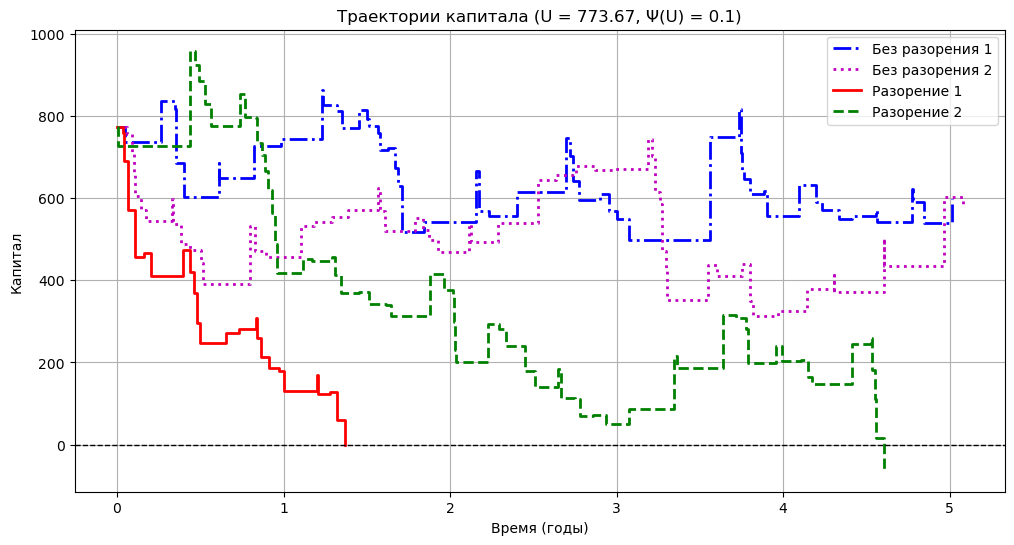
\includegraphics[width=0.95\textwidth]{output.png}
	\label{pic:1}
	\end{figure}
	\subsection*{Выводы}
	\begin{itemize}
		\item Для $\Psi(U)=0.1$ требуется капитал $U \approx 773.7$
		\item При $U=0.2\mathbb{E}Z$ оценка $\Psi(U)$ дает 68.9-71.4\%
		\item Результаты моделирования подтверждают теоретические расчеты
	\end{itemize}
	
	\section*{Задача 4. Модель со стохастическими премиями}
	\subsection*{Исходные параметры}
	\begin{itemize}
		\item Интенсивность премий: $\lambda_1 = 3.0$
		\item Интенсивность убытков: $\lambda = 2.0$
		\item Распределение премий $\eta \sim\Gamma(k_\eta, \theta_\eta) =\Gamma(2, 15)$
		\item Распределение убытков $X \sim\Gamma(k_X, \theta_X) = \Gamma(1.5, 20)$
		\item Целевая вероятность разорения: $\psi(U) = 0.2$
	\end{itemize}
	
	\subsection*{1. Анализ компонентов модели}
	
	\subsubsection*{1.1 Страховые иски $X_i$}
	\begin{equation*}
		\begin{aligned}
			&\text{Плотность: } f_X(x) = \frac{x^{k_X-1}e^{-x/\theta_X}}{\theta_X^{k_X}\Gamma(k_X)} \\
			&\mathbb{E}X = k_X\theta_X = 1.5 \times 20 = 30.0 \\
			&\mathbb{D}X = k_X\theta_X^2 = 1.5 \times 20^2 = 600.0 \\
			&\mathbb{E}X^2 = \mathbb{D}X + (\mathbb{E}X)^2 = 600 + 900 = 1500.0
		\end{aligned}
	\end{equation*}
	
	\subsubsection*{1.2 Число страховых случаев $K(t)$}
	\begin{equation*}
		\begin{aligned}
			&K(t) \sim \text{Poisson}(\lambda t) \\
			&\mathbb{E}K(t) = \lambda t, \quad \mathbb{D}K(t) = \lambda t \\
			&\text{Для } t=1: \quad \mathbb{E}K = 2.0, \quad \mathbb{D}K = 2.0 \\
			&\text{Временные промежутки: } T_i \sim \text{Exp}(\lambda) \\
			&\mathbb{E}T_i = \frac{1}{\lambda} = 0.5 \text{ года}
		\end{aligned}
	\end{equation*}
	
	\subsubsection*{1.3 Суммарный иск $Z(t) = \sum_{i=1}^{K(t)} X_i$}
	\begin{equation*}
		\begin{aligned}
			&\mathbb{E}Z = \mathbb{E}K \cdot \mathbb{E}X = 2 \times 30 = 60.0 \\
			&\mathbb{D}Z = \mathbb{E}K \cdot \mathbb{D}X + \mathbb{D}K \cdot (\mathbb{E}X)^2 \\
			&\quad = 2 \times 600 + 2 \times 900 = 3000.0 \\
			&\sigma_Z = \sqrt{\mathbb{D}Z} \approx 54.77 
			\\
			&\text{Производящая функция: } \phi_Z(s) = e^{\lambda(\phi_X(s)-1)}
		\end{aligned}
	\end{equation*}
	
	\subsubsection*{1.4 Премии $\eta_j$}
	\begin{equation*}
		\begin{aligned}
			&\text{Плотность: } f_\eta(x) = \frac{x^{k_\eta-1}e^{-x/\theta_\eta}}{\theta_\eta^{k_\eta}\Gamma(k_\eta)}\\
			&\mathbb{E}\eta = k_\eta\theta_\eta = 2 \times 15 = 30.0 \\
			&\mathbb{D}\eta = k_\eta\theta_\eta^2 = 2 \times 15^2 = 450.0 \\
			&\mathbb{E}\eta^2 = \mathbb{D}\eta + (\mathbb{E}\eta)^2 = 450 + 900 = 1350.0
		\end{aligned}
	\end{equation*}
	
	\subsubsection*{1.5 Суммарные премии $P(t) = \sum_{j=1}^{M(t)} \eta_j$}
	\begin{equation*}
		\begin{aligned}
			&M(t) \sim \text{Poisson}(\lambda_1 t) \\
			&\mathbb{E}P = \lambda_1\mathbb{E}\eta = 3 \times 30 = 90.0 \\
			&\mathbb{D}P = \lambda_1\mathbb{E}\eta^2 = 3 \times 1350 = 4050.0 \\
			&\sigma_P = \sqrt{4050} \approx 63.64 \\
			&\text{Временные промежутки: } J_j \sim \text{Exp}(\lambda_1) \\
			&\mathbb{E}J_j = \frac{1}{\lambda_1} \approx 0.333 \text{ года}
		\end{aligned}
	\end{equation*}
	
	\subsubsection*{1.6 Коэффициент Крамера $\beta$}
	\begin{equation*}
		\beta = \frac{2(\mathbb{E}P - \mathbb{E}Z)}{\mathbb{D}P + \mathbb{D}Z} = \frac{2(90 - 60)}{4050 + 3000} \approx 0.00857
	\end{equation*}
	
	\subsubsection*{1.7 Расчёт начального капитала}
	\begin{align*}
		&U = -\frac{\ln \psi(U)}{\beta} = -\frac{\ln 0.2}{0.00857} \approx 187.3\\
		&U/\mathbb{E}Z \approx 3.12
	\end{align*}
	
	\subsection*{2. Результаты моделирования}
	После 100 симуляций получены результаты:
		\begin{center}
		\begin{tabular}{cccccc}
			\toprule
			Год & 1 & 2 & 3 & 4 & 5 \\
			\midrule
			Разорения & 1 & 2 & 2 & 1 & 1 \\
			Вероятность & 0.01 & 0.02 & 0.02 & 0.01 & 0.01 \\
			\bottomrule
		\end{tabular}
		\end{center}
		Общая вероятность разорения за пять лет: $\Psi(U) \approx 0.07$.

	\subsection*{3. Визуализация}
		Примеры графиков с разорениями и без разорений:
	\begin{figure}[h]
		\centering
		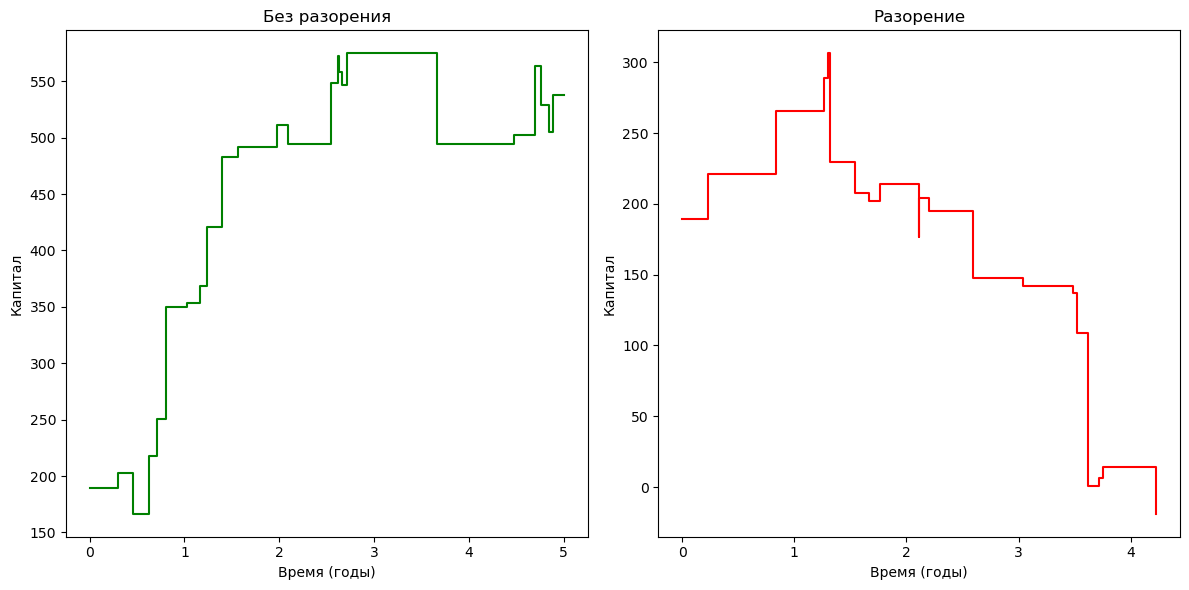
\includegraphics[width=0.8\textwidth]{task4.png}
		\caption{Типичные траектории капитала: (слева) без разорения, (справа) с разорением}
	\end{figure}
	
	\subsection*{Выводы}
	\begin{itemize}
		\item Теоретический расчёт даёт начальный капитал $U \approx 187.3$ для $\psi(U)=0.2$
		\item Отношение $U/\mathbb{E}Z \approx 3.12$ показывает достаточность капитала
	\end{itemize}
\end{document}